\documentclass[10pt]{article}

\usepackage[T1]{fontenc}
\usepackage{newtxtext}
\usepackage{amsthm}
\usepackage{newtxmath}
\usepackage[letterpaper,top=0.72in,bottom=0.76in,left=0.78in,right=0.78in]{geometry}
\usepackage{microtype}
\usepackage{amsmath,mathtools,bm}
\usepackage{booktabs,array,tabularx,multirow}
\usepackage{enumitem}
\usepackage{graphicx}
\usepackage{caption,subcaption}
\usepackage{float}
\usepackage{xcolor}
\usepackage{tikz}
\usetikzlibrary{arrows.meta,positioning,fit,calc,shapes.geometric}
\usepackage[numbers,sort&compress]{natbib}
\usepackage[hidelinks]{hyperref}
\usepackage[nameinlink,noabbrev]{cleveref}
\usepackage{fancyhdr}
\usepackage{lastpage}
\usepackage{titlesec}

\definecolor{vdink}{HTML}{17232D}
\definecolor{vdblue}{HTML}{1D5F8A}
\definecolor{vdorange}{HTML}{B95F2A}
\definecolor{vdgreen}{HTML}{3F7356}
\definecolor{vdred}{HTML}{9F3D45}
\definecolor{vdgray}{HTML}{69747D}
\definecolor{vdpale}{HTML}{EEF2F4}

\hypersetup{
  colorlinks=true,
  linkcolor=vdblue,
  citecolor=vdblue,
  urlcolor=vdblue,
  pdftitle={Emergent Predictive Representation},
  pdfauthor={Logan Voss}
}

\graphicspath{{figures/}}
\setlength{\parindent}{1.15em}
\setlength{\parskip}{0.12em}
\setlist{nosep,leftmargin=1.5em}
\captionsetup{font=small,labelfont=bf}
\titleformat{\section}{\Large\bfseries\color{vdink}}{\thesection}{0.65em}{}
\titleformat{\subsection}{\large\bfseries\color{vdink}}{\thesubsection}{0.55em}{}
\titleformat{\subsubsection}{\normalsize\bfseries\color{vdink}}{\thesubsubsection}{0.5em}{}

\pagestyle{fancy}
\fancyhf{}
\fancyhead[L]{\small\textsc{Emergent Predictive Representation}}
\fancyhead[R]{\small\textsc{Working mathematical thesis}}
\fancyfoot[C]{\small\thepage\ /\ \pageref*{LastPage}}
\renewcommand{\headrulewidth}{0.35pt}

\newtheorem{theorem}{Theorem}[section]
\newtheorem{proposition}[theorem]{Proposition}
\newtheorem{lemma}[theorem]{Lemma}
\newtheorem{corollary}[theorem]{Corollary}
\theoremstyle{definition}
\newtheorem{definition}[theorem]{Definition}
\newtheorem{axiom}[theorem]{Axiom}
\newtheorem{conjecture}[theorem]{Conjecture}
\crefname{axiom}{axiom}{axioms}
\Crefname{axiom}{Axiom}{Axioms}
\theoremstyle{remark}
\newtheorem{remark}[theorem]{Remark}

\newcommand{\E}{\mathbb E}
\newcommand{\R}{\mathbb R}
\newcommand{\C}{\mathbb C}
\newcommand{\Hh}{\mathbb H}
\newcommand{\Tr}{\operatorname{Tr}}
\newcommand{\rank}{\operatorname{rank}}
\newcommand{\sech}{\operatorname{sech}}
\newcommand{\artanh}{\operatorname{artanh}}
\newcommand{\dd}{\mathrm d}
\newcommand{\cI}{\mathcal I}
\newcommand{\cQ}{\mathcal Q}
\newcommand{\cE}{\mathcal E}
\newcommand{\cS}{\mathcal S}
\newcommand{\cD}{\mathcal D}
\newcommand{\cH}{\mathcal H}
\newcommand{\cL}{\mathcal L}
\newcommand{\cR}{\mathcal R}
\newcommand{\cT}{\mathcal T}
\newcommand{\ket}[1]{\lvert #1\rangle}
\newcommand{\bra}[1]{\langle #1\rvert}
\newcommand{\proj}[1]{\lvert #1\rangle\!\langle #1\rvert}
\newcommand{\given}{\,\middle|\,}
\newcommand{\status}[1]{\textsf{\small #1}}

\newcommand{\claimbox}[2]{%
  \begin{center}
  \fcolorbox{vdblue}{vdpale}{%
    \begin{minipage}{0.94\linewidth}
    \textbf{\color{vdink}#1}\quad #2
    \end{minipage}}
  \end{center}}

\begin{document}

\hypersetup{pageanchor=false}
\begin{titlepage}
\thispagestyle{empty}
\vspace*{0.55in}
\noindent{\color{vdblue}\rule{\linewidth}{2.2pt}}
\vspace{0.32in}

{\fontsize{28}{33}\selectfont\bfseries\color{vdink}
Emergent Predictive Representation\par}
\vspace{0.14in}
{\fontsize{16}{21}\selectfont\color{vdgray}
Complex structure, quantum sufficiency, and a one-parameter Hopf-fibre test\par}
\vspace{0.35in}

{\large Logan Voss\par}
\vspace{0.08in}
{\normalsize Voss Dynamics \textbar\ Working mathematical thesis and experimental protocol\par}
\vspace{0.05in}
{\normalsize 21 August 2026\par}

\vfill
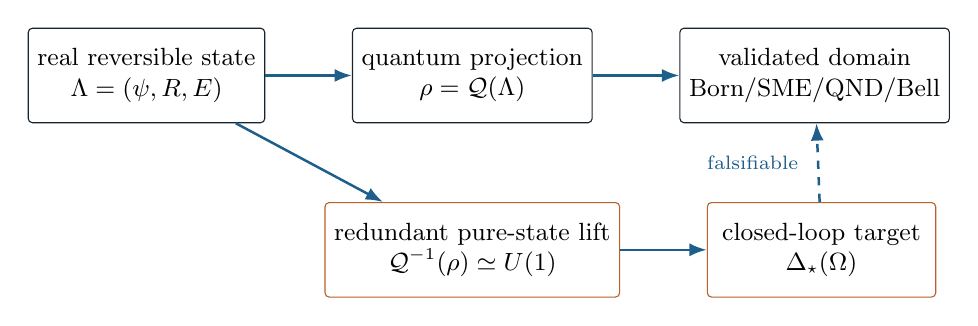
\begin{tikzpicture}[
  node distance=10mm and 11mm,
  every node/.style={font=\small,align=center},
  box/.style={draw=vdink,rounded corners=1.5pt,minimum height=12mm,minimum width=29mm,fill=white},
  arrow/.style={-{Latex[length=2.2mm]},line width=0.9pt,color=vdblue}
]
\node[box] (real) {real reversible state\\$\Lambda=(\psi,R,E)$};
\node[box,right=of real] (proj) {quantum projection\\$\rho=\cQ(\Lambda)$};
\node[box,right=of proj] (qm) {validated domain\\Born/SME/QND/Bell};
\node[box,below=of proj,draw=vdorange] (fiber) {redundant pure-state lift\\$\cQ^{-1}(\rho)\simeq U(1)$};
\node[box,right=of fiber,draw=vdorange] (target) {closed-loop target\\$\Delta_\star(\Omega)$};
\draw[arrow] (real) -- (proj);
\draw[arrow] (proj) -- (qm);
\draw[arrow] (real) -- (fiber);
\draw[arrow] (fiber) -- (target);
\draw[arrow,dashed] (target) --
  node[midway,left=2mm,font=\scriptsize,fill=white,inner sep=1pt]{falsifiable}
  (qm);
\end{tikzpicture}
\vfill

\fcolorbox{vdink}{vdpale}{%
\begin{minipage}{0.94\linewidth}
\textbf{Evidence statement.}
The conditional characterization theorems and reported algebraic identities are proved within their stated assumptions. The numerical results are internal model checks or explicitly labelled synthetic software validations. No laboratory deviation from quantum mechanics is reported. VD-Hopf-1 is a phenomenological ansatz with a memoryless reduced-qubit null at \(\varepsilon=0\), not an established law of nature.
\end{minipage}}

\vspace{0.35in}
\noindent{\color{vdblue}\rule{\linewidth}{0.8pt}}
\end{titlepage}
\hypersetup{pageanchor=true}

\begin{abstract}
This thesis separates an explanatory reconstruction of quantum structure from a test of reduced-state predictive sufficiency. Conditionally on irreducible Euclidean Jordan geometry, a normalized nontrivial stationary real detector reference has a two-dimensional cyclic span. A binary face of Peirce degree \(d\) has an unnormalized reversible QND-filter algebra of dimension \(1+d(d-1)/2\). An explicit accessibility and isomorphism axiom between these spaces forces \(d=2\), selecting the complex Hermitian family. The result is dimension-forcing and conditional; the decisive response-completeness premise is not derived.

For a pure qubit, the redundant lift \(\psi\mapsto\rho=\psi\psi^\dagger\) has a \(U(1)\) Hopf fibre. The ideal QND chart \(s=\artanh z\) yields \(\dd x_\varphi=a\,\dd Y\) and \(\dd c_\varphi=0\), showing that the transverse QND invariant is already encoded in \(\rho\). VD-Hopf-1 therefore postulates instead that a gauge-invariant closed-path holonomy \(\Gamma_{\rm rel}\) survives as physical history memory and enters a later record through
\[
\dd Y_t=a[z_t+\varepsilon(1-z_t^2)\sin\Gamma_{{\rm rel},t}]\dd t+\dd W_t .
\]
Mirror loops give a leading orientation-odd sine law. The memoryless reduced-qubit null is \(\varepsilon=0\).

All quantum-limit checks and synthetic statistics are internal regressions. No memory carrier, mixed/composite instrument, or beyond-quantum result is derived or observed. The experimental deliverable is a draft bounded-model protocol: a positive result would first show unexplained history dependence relative to specified reduced-qubit, qutrit--cavity, and finite-memory models.
\end{abstract}

\claimbox{Primary result}{The defensible mathematical refinement is a \emph{fibre distinction}: the QND transverse invariant is hidden from one record but encoded in the quantum state; a normalized pure-spinor lift has a redundant \(U(1)\) fibre. VD-Hopf-1 separately postulates a gauge-invariant holonomy memory and asks whether a protocol-fixed matched-state variation is nonzero.}

\tableofcontents
\clearpage

\section{Question, standard of proof, and the six courts}

\subsection{The thesis in one equation}

Let \(\Lambda\) denote a complete candidate state, \(A\) an intervention, and \(O\) its outcome. Because ``EPR'' conventionally denotes Einstein--Podolsky--Rosen in quantum foundations, this manuscript writes \emph{Emergent Predictive Representation} in full and calls the concrete ansatz VD-Hopf-1. The proposition is that a map
\begin{equation}
  \rho=\cQ(\Lambda)
  \label{eq:projection}
\end{equation}
reproduces the successful quantum domain but may be predictively lossy. Conditional mutual information requires a preparation prior. For an admissible prior \(\mu\) on \(\Lambda\) and bounded intervention class \(\mathcal A\), define
\begin{equation}
  \cE(\mu,\mathcal A)
  :=
  \sup_{\mathsf a\in\mathcal A}
  I_\mu(\Lambda;O\mid \rho,A=\mathsf a),
  \label{eq:latent-defect}
\end{equation}
and, if needed, maximize over a declared admissible prior family \(\mathfrak M\). A model-level separating pair obeys
\begin{equation}
  \Lambda_+\neq\Lambda_-,
  \qquad
  \cQ(\Lambda_+)=\cQ(\Lambda_-)=\rho,
  \qquad
  P(O\mid\mathsf a,\Lambda_+)
  \neq
  P(O\mid\mathsf a,\Lambda_-).
  \label{eq:golden-pair}
\end{equation}
Because \(\Lambda\) is not directly observed, \cref{eq:latent-defect} is prior-dependent and theoretical. The total-variation objective later is the primary prior-free model criterion, and the estimable witness replaces \(\Lambda\) by randomized preparation histories. A same-reduced-\(\rho\) pair establishes reduced-state insufficiency; it does not by itself exclude an enlarged standard quantum state.

\subsection{Claim discipline}

Four statuses are used throughout:
\begin{description}[style=nextline]
\item[\status{PROVED}] A mathematical consequence of explicitly listed assumptions.
\item[\status{COMPUTED}] A symbolic or numerical identity reproduced by code and tests.
\item[\status{CANDIDATE}] A specified law that is consistent enough to test but is not inferred from physical data.
\item[\status{OPEN}] A physical or novelty claim requiring experiment, stronger axioms, or independent literature confirmation.
\end{description}
No synthetic dataset can establish that Nature implements a candidate mechanism. No fit to an unsealed target counts as a prediction. A reconstruction of standard quantum mechanics is not evidence against standard quantum mechanics.

\subsection{Court ledger}

\begin{table}[H]
\centering
\caption{The six courts and their present status. The ledger deliberately separates conditional mathematics, baseline checks, candidate definitions, and open physical work.}
\label{tab:courts}
\small
\begin{tabularx}{\linewidth}{@{}p{0.08\linewidth}X p{0.28\linewidth}@{}}
\toprule
Court & Required object & Result in this thesis\\
\midrule
1 & Small admissible real geometry under strengthened reversibility, stationary reference, QND calibration, covariance, causality, mixing, and no-signalling constraints. & \status{CONDITIONAL}: reference and filter-stabilizer lemmas; dimension-forcing accessibility/completeness axiom remains.\\
2 & A map \(\cQ:(\xi,R,E)\mapsto\rho\), with phase structure identified rather than renamed. & \status{PARTIAL}: exact redundant pure-spinor lift and QND chart; no derived physical fibre ontology or canonical mixed-state fibre.\\
3 & Born probabilities, unitaries, trajectories, phase backaction, dephasing, Rabi, Zeno, two-qubit correlations, CHSH, and no-signalling. & \status{BASELINE CHECK}: exact at \(\varepsilon=0\); not an independent derivation of the full instrument calculus.\\
4 & Lowest-order departures surviving declared symmetries. & \status{CANDIDATE}: one chosen basis element; no complete mixed/composite instrument.\\
5 & Two deeper states with the same matched projected state and different predictions. & \status{MODEL-CONDITIONAL}: same reduced \(\rho\), opposite holonomy label, and nonzero ansatz drift; physical memory carrier is postulated.\\
6 & Frozen target, likelihood, calibration boundary, controls, and failure rule. & \status{DRAFT}: synthetic Gaussian summary validation; bounded process tensor, qutrit--cavity null, path score, thresholds, and external commitment remain open.\\
\bottomrule
\end{tabularx}
\end{table}

\section{Court 1: admissible state geometry}

\subsection{Operational state before ontology}

Let \(h\) be a complete available preparation history. Two histories are operationally equivalent when no allowed future intervention distinguishes them:
\begin{equation}
  h\sim h'
  \iff
  P(o\mid\operatorname{do}(a),h)
  =
  P(o\mid\operatorname{do}(a),h')
  \quad \forall\,a,o.
  \label{eq:predictive-equivalence}
\end{equation}
An operational state is the class \([h]\). Independent classical randomization makes the normalized state set convex, and effects are affine probability functionals. This is standard operational-probabilistic structure, not yet quantum theory.

The finite-dimensional homogeneous self-dual (HSD) cone assumption is substantial. By the Koecher--Vinberg correspondence, an HSD cone is the cone of squares of a Euclidean Jordan algebra (EJA) \citep{Koecher1957,Vinberg1963,FarautKoranyi1994}. Modern work seeks operational replacements for self-duality \citep{Barnum2023}; this thesis does not claim to have removed that premise.

\begin{axiom}[Jordan domain]
\label{ax:jordan}
The finite-dimensional unnormalized operational states form an irreducible homogeneous self-dual cone of rank \(r\ge2\). Equivalently, they are represented by an irreducible EJA \(J\) with binary faces.
\end{axiom}

The Jordan--von Neumann--Wigner classification contains real, complex, and quaternionic Hermitian matrix algebras, spin factors, and the exceptional \(3\times3\) octonionic algebra \citep{Jordan1934,FarautKoranyi1994}. The task is therefore not to rediscover that list, but to identify an observation principle that selects one member.

\subsection{Measure preservation excludes positive-measure attraction}

\begin{proposition}[No positive-measure attraction in a measure-preserving flow]
\label{prop:no-attractor}
Let \(X\) be a metric space with a finite regular Borel measure \(\mu\), and let \(\Psi_t\) be an invertible measure-preserving flow. If \(A\subset X\) is closed with \(\mu(A)=0\), there is no measurable \(B\) with \(\mu(B)>0\) that is uniformly attracted to \(A\), meaning that for every open neighborhood \(N\supset A\) there is \(t_N\) such that \(\Psi_t(B)\subset N\) for all \(t\ge t_N\).
\end{proposition}

\begin{proof}
Regularity and \(\mu(A)=0\) give an open \(N\supset A\) with \(\mu(N)<\mu(B)\). Uniform attraction would eventually imply \(\Psi_t(B)\subset N\), whereas measure preservation gives \(\mu(\Psi_tB)=\mu(B)>\mu(N)\), a contradiction.
\end{proof}

Invertibility by itself does not imply this result: \(\dot x=-x\) has an invertible finite-time flow and contracts. The Voss architecture therefore needs measure preservation, Hamiltonian/unitary structure, or another explicit conservation law in addition to reversibility if damping and stochastic collapse are to be reduced descriptions only. Under that strengthened baseline, a complete candidate state retains system, reference, and environment variables,
\begin{equation}
  \Lambda=(\xi,R,E),\qquad
  \Lambda_{t+\Delta t}=\Psi_{\Delta t}(\Lambda_t),
  \qquad \Psi_{\Delta t}^{-1}\ \text{exists}.
  \label{eq:reversible-lift}
\end{equation}
Unitary system--field dilation is an established way to realize this logic for quantum filters \citep{Bouten2007,WisemanMilburn2010}. Reversibility alone does not determine \(\Psi\).

\subsection{Smallest symmetry-forced generator class}

Court 1 asks for the smallest \(F\), not an invented damping field. On a finite-dimensional real complete state \(X\) with stationary quadratic calibration \(\|X\|^2\), assume a local linear control law
\[
\dot X=A(u)X.
\]
Stationarity for every \(X\) gives
\[
\frac{\dd}{\dd t}\|X\|^2
=X^\mathsf T[A(u)^\mathsf T+A(u)]X=0,
\]
and therefore
\begin{equation}
  A(u)^\mathsf T=-A(u).
  \label{eq:minimal-skew-generator}
\end{equation}
Thus the minimal closed linear class is orthogonal transport,
\[
F_0(X,u)=A(u)X,\qquad A(u)\in\mathfrak{so}(N),
\]
with no contraction coefficient. The elementary spinor requires \(X_\psi\in S^3\subset\R^4\); the reference theorem below supplies a real rotation block; measurement requires additional environment/field coordinates. Conditioning or tracing those coordinates can yield a stochastic master equation, but reduced damping is not inserted into \(F_0\).

This is a classification only within the declared linear stationary class. General reversible nonlinear dynamics may be Hamiltonian,
\(\dot X=\mathbb J\nabla H(X,u)\), and are not uniquely fixed by the present axioms. The thesis therefore uses the smallest linear lift as the baseline and parameterizes every proposed departure explicitly.

\subsection{Minimal real reference}

Let \(W\) be a finite-dimensional real detector-reference space with its calibrated covariance inner product. Let \(P\in W\) be a centered real pointer and let changing the reference origin act by a strongly continuous one-parameter group \(R_s\).

\begin{axiom}[Stationary cyclic reference]
\label{ax:reference}
\(P\) is normalized, \(\|P\|=1\); \(R_s\) preserves the covariance inner product; the action is nontrivial on \(P\), so \(R_sP\neq P\) for some \(s\); and the cyclic subspace
\[
W_P=\operatorname{span}\{R_sP:s\in\R\}
\]
is irreducible under \(R_s\).
\end{axiom}

\begin{theorem}[Minimal real reference]
\label{thm:minimal-reference}
Under \cref{ax:reference}, \(\dim W_P=2\). There are orthonormal \(P,Q\) and \(\omega>0\) such that
\begin{equation}
  R_sP=P\cos(\omega s)+Q\sin(\omega s).
  \label{eq:reference-rotation}
\end{equation}
The normalized orbit is \(S^1\), and \(J_R:=A/\omega\) obeys \(J_R^2=-I\) on \(W_P\).
\end{theorem}

\begin{proof}
Stationarity gives \(R_s\in O(W)\). Strong continuity gives \(R_s=e^{sA}\), and differentiating \(R_s^\mathsf TR_s=I\) yields \(A^\mathsf T=-A\). Every real skew-symmetric operator is an orthogonal direct sum of zero blocks and two-dimensional rotation blocks. Nontriviality excludes a zero block; irreducibility excludes more than one block. Hence \(W_P\) is one rotation plane. Choosing \(Q=AP/\omega\) gives \cref{eq:reference-rotation} and \(J_R^2=-I\).
\end{proof}

The theorem is elementary representation theory. Its relevance is physical only if \(W_P\) is independently calibrated and its response to the system is not postulated to have the desired dimension.

\subsection{Binary Jordan faces and their unnormalized QND-filter stabilizer}

Let \(p,q\) be orthogonal primitive idempotents. Their rank-two face has Peirce decomposition
\begin{equation}
  J[p,q]=\R p\oplus\R q\oplus J_{pq},
  \qquad d:=\dim J_{pq}.
  \label{eq:peirce-face}
\end{equation}
Every rank-two EJA is a spin factor. Its unnormalized cone can be written as the Lorentz cone
\begin{equation}
  \cL_{d+2}
  =
  \left\{(t,z,\bm c):
  t\ge 0,\ t^2\ge z^2+\|\bm c\|^2,\ \bm c\in\R^d
  \right\},
  \label{eq:lorentz-cone}
\end{equation}
with QND outcome rays
\(\ell_\pm=\R_{\ge0}(1,\pm1,\bm0)\).

\begin{lemma}[Unnormalized QND-filter stabilizer]
\label{lem:qnd-stabilizer}
Modulo global cone dilation, the connected Lie algebra of linear Lorentz-cone automorphisms preserving each ray \(\ell_+\) and \(\ell_-\) is
\begin{equation}
  \mathfrak f_{pq}
  \cong
  \R K_{pq}\oplus\mathfrak{so}(d),
  \qquad
  \dim\mathfrak f_{pq}=1+\frac{d(d-1)}{2}.
  \label{eq:qnd-algebra}
\end{equation}
\end{lemma}

\begin{proof}
The connected cone automorphism algebra is
\(\R I\oplus\mathfrak{so}(1,d+1)\). Requiring an infinitesimal generator to map both null rays into themselves removes boosts mixing \((t,z)\) with \(\bm c\) and removes null rotations. After quotienting the central dilation, the remaining blocks are the single \(t\)--\(z\) boost \(K_{pq}\) and arbitrary rotations of \(\bm c\), namely \(\mathfrak{so}(d)\). The dimension follows.
\end{proof}

The word ``reversible'' here means invertible as an unnormalized cone order-automorphism. The boost \(K_{pq}\) changes the order unit and is a probabilistically reversible filter/measurement branch, not a deterministic reversible channel on normalized states. Quotienting \(\mathbb RI\) is appropriate only for normalized conditional-state transformations; the overall branch scale remains relevant to raw outcome probability and must be calibrated separately. The normalized deterministic stabilizer would retain only \(\mathfrak{so}(d)\), and the dimension argument below would not follow.

\subsection{Conditional complex-scalar characterization}

Detector reference directions need not automatically equal system generator directions. The bridge is isolated as an axiom rather than hidden in the prose.

\begin{axiom}[Accessible, faithful, and generator-complete filter response]
\label{ax:complete-response}
Every vector in the two-dimensional linear span \(W_P\), not merely the tangent to its one-parameter orbit, is assumed to be an independently accessible infinitesimal detector perturbation. ``Complete'' means direct first-order linear spanning, not reachability generated by sequential controls or Lie brackets. For every binary face these perturbations induce a linear response
\[
\Phi_{pq}:W_P\longrightarrow\mathfrak f_{pq}
\]
that is injective (no accessible detector direction is idle) and surjective (no unnormalized reversible QND-filter generator is inaccessible).
\end{axiom}

\begin{theorem}[Conditional detector/filter complex-scalar characterization]
\label{thm:complex-scalar}
Let \(J\) satisfy \cref{ax:jordan}. If \cref{ax:reference,ax:complete-response} hold for every binary face, then
\[
J\simeq H_r(\C)_{\mathrm{sa}}.
\]
For rank two, the state space is the ordinary complex qubit.
\end{theorem}

\begin{proof}
\Cref{thm:minimal-reference} gives \(\dim W_P=2\). Faithfulness and completeness make \(\Phi_{pq}\) an isomorphism, so \(\dim\mathfrak f_{pq}=2\). By \cref{lem:qnd-stabilizer},
\[
2=1+\frac{d(d-1)}2.
\]
The only nonnegative integer solution is \(d=2\). The classification of irreducible EJAs then leaves the complex Hermitian series; the rank-two spin factor at \(d=2\) is \(H_2(\C)_{\mathrm{sa}}\).
\end{proof}

The proof uses only vector-space dimension. A generic bijection \(\Phi_{pq}\) need not be isometric, need not map the detector quarter-turn \(J_R\) to the canonical system complex structure, and can map a detector circle to an ellipse. Any stronger identification of the physical meaning of \(i\) requires an additional equivariance or calibration theorem.

\begin{figure}[H]
\centering
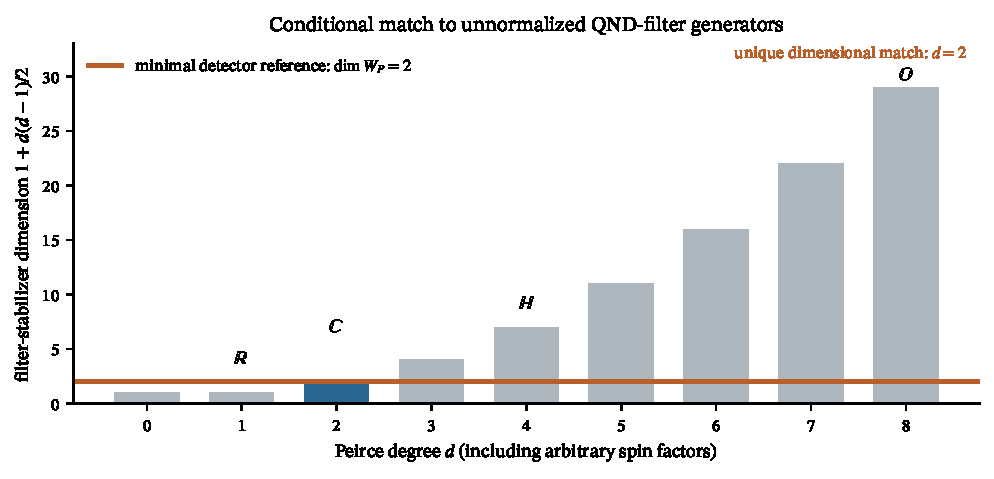
\includegraphics[width=0.78\linewidth]{scalar_selection.pdf}
\caption{The detector-reference span and unnormalized QND-filter stabilizer dimension agree only at Peirce degree \(d=2\). Arbitrary integer degrees, including rank-two spin factors, are shown. The visual does not weaken the logical qualification: accessibility, injectivity, and surjectivity of \(\Phi_{pq}\) are assumptions.}
\label{fig:scalar-selection}
\end{figure}

\paragraph{Novelty boundary.}
The EJA classification, Koecher--Vinberg theorem, Peirce geometry, and Lorentz-cone groups are established mathematics \citep{Jordan1934,FarautKoranyi1994}. Local tomography plus Jordan structure and a qubit already selects ordinary complex quantum theory under additional factorizable-self-duality and composite-system assumptions \citep{BarnumWilce2014}; energy observability and dynamical correspondence provide neighboring complex selectors \citep{BarnumMullerUdudec2014,Niestegge2015}; reversible filters are also established reconstruction machinery \citep{Wilce2019}. The potentially distinct contribution here is only the \emph{specific conditional dimension-matching criterion} between a minimal real detector-reference span and the complete unnormalized QND-filter algebra. The one-parameter orbit itself has a one-dimensional tangent; treating both vectors in \(W_P\) as independently accessible perturbations is part of \cref{ax:complete-response}, not a consequence of \cref{thm:minimal-reference}. Until peer-reviewed novelty audit and derivation of that axiom are complete, the result must not be described as ``observation alone proves \(\C\).''

\subsection{Causality, mixing, and no-signalling}

Operational causality requires normalized probabilities for every deterministic test and forbids dependence on future interventions. Classical randomization is affine at the level of probability measures on \(\Lambda\):
\[
\mu=\lambda\mu_1+(1-\lambda)\mu_2
\quad\Longrightarrow\quad
P(o\mid a,\mu)
=\lambda P(o\mid a,\mu_1)+(1-\lambda)P(o\mid a,\mu_2).
\]
At \(\varepsilon=0\), the complex quantum representation and tensor product recover standard no-signalling. If different preparation histories with the same operational state produced different future laws, the model would be preparation contextual in the generalized sense \citep{Spekkens2005}; its bipartite extension is not licensed by single-system equations. \Cref{sec:no-signalling} states the operational constraint relevant to the Gisin--Polchinski signalling mechanism \citep{Gisin1990,Polchinski1991}.

\section{Court 2: explicit quantum representation and redundant lift}

\subsection{From a real rotation plane to a complex structure}

On the detector reference plane, \(J_R^2=-I\). The notation
\[
u+iv
\quad\longleftrightarrow\quad
uI+vJ_R
\]
is therefore a compression of a real two-dimensional rotation. This explains how a complex structure can be represented by real relational geometry; it does not show that every physically allowed transformation must commute with the same \(J_R\).

Given \cref{thm:complex-scalar}, an elementary pure state is a rank-one projector that \emph{can be represented redundantly} by a normalized two-component complex spinor
\(\psi=(\alpha,\beta)^\mathsf T\in S^3\subset\R^4\). The EJA theorem yields the projector/ray, not a physical point of \(S^3\). The representative map is
\begin{equation}
  \boxed{\quad
  \cQ(\psi)=\psi\psi^\dagger
  =\frac12(I+\bm r\cdot\bm\sigma).
  \quad}
  \label{eq:hopf-projection}
\end{equation}
This is the Hopf fibration \(S^1\hookrightarrow S^3\to S^2\) \citep{MosseriDandoloff2001}. It is invariant under
\begin{equation}
  \psi\mapsto e^{i\chi}\psi.
  \label{eq:fibre-action}
\end{equation}
Thus the fibre \(\cQ^{-1}(\rho)\) within the normalized pure-spinor lift is \(U(1)\).

\begin{figure}[H]
\centering
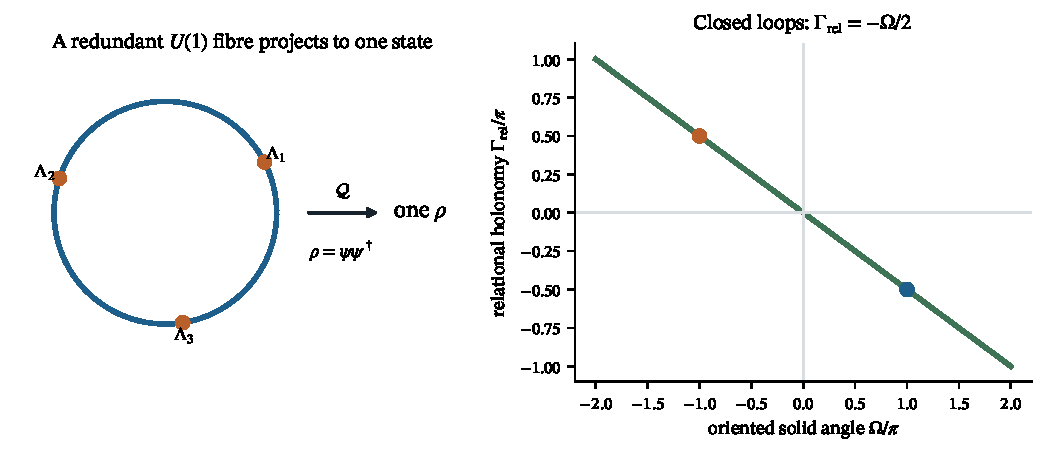
\includegraphics[width=0.92\linewidth]{hopf_projection.pdf}
\caption{Left: many spinors on one \(U(1)\) fibre project to the same density matrix. Right: the natural spin-\(\tfrac12\) connection produces closed-loop holonomy \(\Gamma_{\rm rel}=-\Omega/2\). Standard quantum mechanics predicts no system-only distinction after the same ray is restored; any physical reference must be included in the declared bounded enlarged-quantum null.}
\label{fig:hopf}
\end{figure}

The Hopf representation is standard, and retaining the full \(S^3\) geometry or debating physical significance of the discarded phase is not new \citep{MosseriDandoloff2001,WhartonKoch2015}. The distinct candidate contribution sought here is narrower: formulate a matched protocol-level variation objective, isolate a gauge-invariant closed-history label, and freeze a future nominally QND record ansatz that standard enlarged quantum models must try to explain.

\subsection{Exact relational chart}

Choose a local gauge with \(\alpha>0\) and define
\begin{equation}
  \frac{\beta}{\alpha}=e^{-s+i\vartheta},
  \qquad s\in\R,\quad\vartheta\in S^1.
  \label{eq:ratio}
\end{equation}
Then
\begin{equation}
  \bm r(s,\vartheta)
  =
  \left(
  \sech s\cos\vartheta,\,
  \sech s\sin\vartheta,\,
  \tanh s
  \right),
  \label{eq:relational-bloch}
\end{equation}
and
\begin{equation}
  \rho(s,\vartheta)
  =
  \frac12
  \begin{pmatrix}
  1+\tanh s & \sech s\,e^{-i\vartheta}\\
  \sech s\,e^{i\vartheta} & 1-\tanh s
  \end{pmatrix}.
  \label{eq:relational-density}
\end{equation}
The poles are obtained as \(s\to\pm\infty\). Mixed states are convex mixtures, or equivalently
\[
\rho_{\nu,s,\vartheta}
=\tfrac12[I+\nu\bm r(s,\vartheta)\cdot\bm\sigma],
\qquad 0\le\nu\le1,
\]
but this chart is nonunique at \(\nu=0\), and a mixed density operator has no canonical \(U(1)\) Hopf fibre. Purification, Uhlmann, and interferometric holonomies are different structures \citep{Uhlmann1986,Sjoqvist2000}.

The complete real candidate coordinate can be written
\begin{equation}
  \Lambda=(s,\vartheta,\chi,E),
  \qquad
  \psi(\Lambda)
  =
  \frac{e^{i\chi}}{\sqrt{1+e^{-2s}}}
  \begin{pmatrix}1\\e^{-s+i\vartheta}\end{pmatrix}.
  \label{eq:deep-spinor}
\end{equation}
The explicit effective map used here is
\begin{equation}
  \cQ(s,\vartheta,\chi,\nu)
  :=
  \rho_{\nu,s,\vartheta}.
  \label{eq:mixed-projection}
\end{equation}
At \(\nu=1\) this is the Hopf projection of \cref{eq:deep-spinor}; for \(\nu<1\), \(\chi\) is only a redundant coordinate attached by this parameterization, not a canonical mixed-state fibre.

In the notation \(\Lambda=(\xi,R,E)\), one may take
\[
\xi=s,\qquad
R=(e^{i\vartheta},e^{i\chi}),\qquad
E\supset\nu,
\]
where the first circle is the component-relative phase relation, the second is the mathematical Hopf fibre, and \(\nu\) records reduced purity. This is a coordinate decomposition, not a claim that both circles are independently observable. The later candidate replaces bare \(\chi\) by the gauge-invariant closed-history memory \(\Gamma_{\rm rel}[C]\).

The effective state \(\rho=\cQ(\Lambda)\) forgets \(\chi\). In relational language, \(\vartheta\) is the phase between spinor components; \(\chi\) is the phase of the whole spinor relative to an external reference. Quantum reference-frame theory warns that a physical reference is itself a quantum system and that only invariant relational quantities are observable \citep{Bartlett2007,Loveridge2018}. This warning is central to the null model.

Accordingly, VD-Hopf-1 below is restricted to conditioned pure, efficient trajectories (\(\nu=1\)) and is only a phenomenological record ansatz. A hardware protocol must either enforce a preregistered near-purity/no-jump slice with quantified selection bias or first supply a mixed-state or purification-level holonomy law. The present thesis does not contain that extension.

\subsection{The ideal QND chart}

For an efficient phase-sensitive \(Z\)-QND measurement, take the normalized It\^o model
\begin{align}
  \dd Y_t&=a\cos\varphi\,z_t\,\dd t+\dd W_t,
  \label{eq:qnd-record}\\
  \dd z_t&=a\cos\varphi(1-z_t^2)\,\dd W_t,
  \label{eq:qnd-z}\\
  \dd\vartheta_t
  &=a\sin\varphi\,\dd W_t
  +a^2\sin\varphi\cos\varphi\,z_t\,\dd t .
  \label{eq:qnd-theta}
\end{align}
Factors depend on measurement-strength convention; the identities below are convention-consistent. Circuit-QED quantum Bayesian and filtering treatments contain precisely the split between informational and phase backaction controlled by homodyne angle \citep{Korotkov2011,Gambetta2008,Hatridge2013}.

Let \(s=\artanh z\). It\^o's lemma gives
\begin{equation}
  \dd s_t=a\cos\varphi\,\dd Y_t,
  \qquad
  \dd\vartheta_t=a\sin\varphi\,\dd Y_t.
  \label{eq:qnd-linear}
\end{equation}
Define
\begin{align}
  x_\varphi&=s\cos\varphi+\vartheta\sin\varphi,\\
  c_\varphi&=-s\sin\varphi+\vartheta\cos\varphi.
\end{align}
Then
\begin{equation}
  \boxed{\quad
  \dd x_\varphi=a\,\dd Y_t,\qquad
  \dd c_\varphi=0.
  \quad}
  \label{eq:qnd-translation}
\end{equation}
Equivalently,
\(\chi_{\rm QND}=\vartheta-\tan\varphi\,\artanh z
=c_\varphi/\cos\varphi\)
is conserved where \(\cos\varphi\neq0\). The supplied blind symbolic program recovered both the invariant and the observable quotient with zero It\^o residual; its control search also recovered the local D-optimal axis \(|n_z|=1/\sqrt3\). These are checks of known quantum dynamics, not beyond-quantum evidence.

The construction is local: \(\vartheta\) is unwrapped on a chart, whereas the physical phase is periodic, and the poles require separate coordinates. It is not a global orthogonal coordinate system on the Bloch sphere.

\begin{figure}[H]
\centering
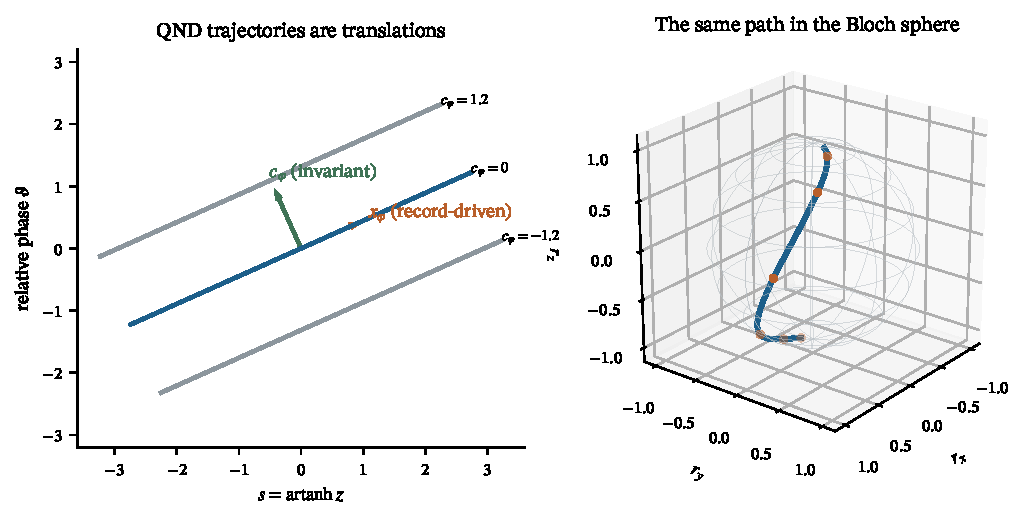
\includegraphics[width=\linewidth]{relational_geometry.pdf}
\caption{The nonlinear pure-state QND trajectory becomes a straight translation in \((s,\vartheta)\). The record determines position along a line; \(c_\varphi\) labels which line. The right panel maps one line back to the Bloch sphere.}
\label{fig:qnd-geometry}
\end{figure}

\subsection{Fibre distinction theorem}

\begin{theorem}[QND transverse information is not fibre information]
\label{thm:fibre-distinction}
On any chart where \((s,\vartheta)\leftrightarrow\rho\) is one-to-one, \(c_\varphi\) is a function of \(\rho\) and the known setting \(\varphi\). Therefore two states satisfying \(\cQ(\Lambda_1)=\cQ(\Lambda_2)\) cannot differ in \(c_\varphi\). By contrast, they may differ in the Hopf coordinate \(\chi\).
\end{theorem}

\begin{proof}
\Cref{eq:relational-density} recovers \(z=\Tr(\rho\sigma_z)\), hence \(s=\artanh z\), and recovers \(\vartheta=\arg\rho_{10}\) away from the poles. Thus \(c_\varphi=-s\sin\varphi+\vartheta\cos\varphi\) is fixed by \(\rho\) and \(\varphi\). \Cref{eq:hopf-projection,eq:fibre-action} show that \(\chi\) is not.
\end{proof}

This theorem changes the experimental target. The QND invariant is important for control and observability, but assigning it to a reference cannot by itself make \(\rho\) predictively incomplete. A Court-5 variable must distinguish points in a fibre of \(\cQ\); the smallest connected fibre in the chosen normalized pure-spinor lift is \(U(1)\).

\section{Court 3: recovery of validated quantum limits}

\subsection{Born effects and an explicit logical boundary}

Once the complex positive cone is adopted, every affine effect has the form
\begin{equation}
  e_M(\rho)=\Tr(\rho M),
  \qquad 0\le M\le I.
  \label{eq:born-effect}
\end{equation}
Sharp calibration to a primitive outcome gives \(M=\Pi_k\), hence
\begin{equation}
  P(k\mid\rho)=\Tr(\rho\Pi_k).
  \label{eq:born}
\end{equation}
This is the Born rule in the reconstructed representation. Gleason-type results explain the measure structure, with generalized effects including the qubit case \citep{Gleason1957,Busch2003}. It would be circular to call \cref{eq:born} a derivation from basin volumes if affinity or effect structure had already inserted the quantum probability functional. The present result is therefore: \emph{conditional scalar reconstruction plus affine effects recovers Born probabilities}; it is not a non-quantum dynamical proof of Born's rule.

\subsection{Unitary and continuous-measurement dynamics}

For \(H=\frac{\hbar}{2}\bm\omega\cdot\bm\sigma\),
\begin{equation}
  \dot\rho=-\frac{i}{\hbar}[H,\rho]
  \quad\Longleftrightarrow\quad
  \dot{\bm r}=\bm\omega\times\bm r.
\end{equation}
This is a reversible \(SO(3)\) action on the Bloch ball and an \(SU(2)\) lift on \(S^3\). A standard efficient diffusive measurement of \(Z\) can be written
\begin{equation}
  \dd\rho
  =
  -\frac{i}{\hbar}[H,\rho]\dd t
  +\Gamma_m\cD[\sigma_z]\rho\,\dd t
  +\sqrt{\eta\Gamma_m}\,
  \cH[e^{-i\varphi}\sigma_z]\rho\,\dd W ,
  \label{eq:sme}
\end{equation}
where
\[
\cD[L]\rho=L\rho L^\dagger-\tfrac12\{L^\dagger L,\rho\},
\qquad
\cH[L]\rho=L\rho+\rho L^\dagger
-\Tr[(L+L^\dagger)\rho]\rho.
\]
The innovations filter follows from quantum conditional expectation and system--field dilation \citep{Bouten2007,WisemanMilburn2010}. Experimental quantum trajectories and variable quadrature backaction are established \citep{Murch2013,Hatridge2013,deLange2014,Atalaya2019}.

\subsection{Dephasing, Rabi dynamics, and the Zeno limit}

Unobserved measurement dephases transverse coherence,
\[
\rho_{01}(t)=\rho_{01}(0)e^{-\Gamma_\phi t},
\]
while a transverse drive produces Rabi rotation. For strong \(Z\)-measurement dephasing \(\Gamma_m\gg\Omega_R\), transitions generated by a noncommuting drive are suppressed: the quantum Zeno limit. Circuit-QED trajectory theory derives both quantum jumps and this suppression \citep{Gambetta2008}. The computations used here exponentiate the Bloch generator, rather than infer the effect from a plot.

\subsection{Two qubits, CHSH, and no-signalling}

With the standard locally tomographic complex composite, the singlet state is
\begin{equation}
  \rho_-=\frac14
  \left(
  I\otimes I-\sum_{j=x,y,z}\sigma_j\otimes\sigma_j
  \right).
\end{equation}
Projective outcomes \(a,b\in\{\pm1\}\) along unit vectors \(\bm x,\bm y\) have
\begin{align}
  P(a,b\mid\bm x,\bm y)
  &=\frac14[1-ab\,\bm x\cdot\bm y],\\
  E(\bm x,\bm y)&=-\bm x\cdot\bm y.
\end{align}
The standard CHSH settings give
\begin{equation}
  |S_{\mathrm{CHSH}}|=2\sqrt2
  \label{eq:chsh}
\end{equation}
and
\(\sum_bP(a,b\mid\bm x,\bm y)=1/2\), independent of \(\bm y\). Bell locality is violated, while operational no-signalling is retained \citep{Bell1964,CHSH1969,Tsirelson1980}. Loophole-free tests establish the physical severity of this constraint \citep{Shalm2015,Giustina2015}.

\begin{figure}[H]
\centering
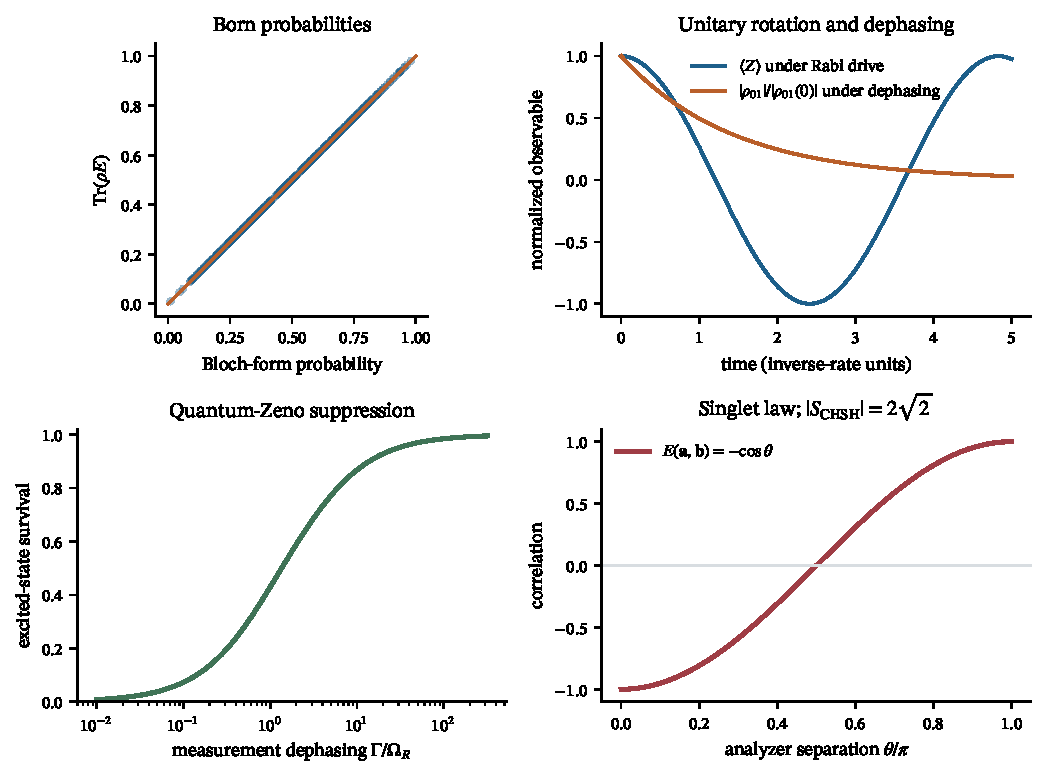
\includegraphics[width=\linewidth]{quantum_limits.pdf}
\caption{Internal regression checks for Court 3. The Born trace identity, unitary/dephasing laws, Zeno suppression, singlet correlation, Tsirelson value, and no-signalling marginals agree with their encoded exact values to floating-point precision.}
\label{fig:qm-limits}
\end{figure}

\subsection{What ``recover'' means}

At \(\varepsilon=0\), the candidate is exactly the standard complex-qubit representation and therefore inherits all results above. This is a valid embedding, not an independent derivation of every quantum instrument from weaker real dynamics. Court 3 is closed as a \emph{consistency and limit} court. A stronger reconstruction would need to derive the full completely positive instrument calculus and composition rule without assuming them.

\section{Court 4: the first allowed departure}

\subsection{Why a new variable must live in a projection fibre}

Suppose a correction depends only on \(\rho\), the intervention, and calibrated environment variables. It is then a modified quantum-state law, but not evidence that \(\cQ\) is lossy. Court 5 demands dependence on a variable \(u\) with
\(\cQ(\rho,u)=\rho\).
For pure qubits, \cref{thm:fibre-distinction} identifies the smallest connected mathematical option as the coordinate \(\gamma\in U(1)\).

The physical candidate is \emph{not} an observable absolute global phase. It is a relational memory of a closed preparation history. For a loop \(C\), define
\begin{equation}
  \Gamma_{\rm rel}[C]
  :=
  \oint_C\mathcal A
  \pmod{2\pi},
  \qquad
  \mathcal A=+i\langle\psi\mid\dd\psi\rangle ,
  \label{eq:relative-fibre}
\end{equation}
for a periodic lift, after dynamical phase and the physical reference path are included or canceled \citep{Simon1983,SamuelBhandari1988}. For a nonperiodic gauge one must include the endpoint Pancharatnam term. Under a periodic gauge change, the closed integral changes only by \(2\pi\mathbb Z\), so every function of \(e^{i\Gamma_{\rm rel}}\) is gauge invariant. The local candidate state is therefore written
\[
\Lambda=(\rho,\Gamma_{\rm rel},\eta),
\]
where \(\eta\) denotes all matched standard quantum reference, environment, leakage, and process variables. This is not ``a wavefunction with observable global phase.''

\begin{conjecture}[Holonomy-memory postulate]
\label{conj:holonomy-memory}
There exists a physical carrier for \(\Gamma_{\rm rel}[C]\) that survives the declared delay/reset operation, while all variables represented in the frozen bounded standard-quantum process state \(\eta\) are matched between mirror histories within specified confidence margins. Unrepresented modes remain a limitation. Geometry alone does not imply this.
\end{conjecture}

\subsection{Symmetry truncation}

We seek a correction \(g(z,\Gamma_{\rm rel})\) to a static \(Z\)-QND scalar record. The declared leading-order class obeys:
\begin{enumerate}[label=(S\arabic*)]
\item \textbf{Reference covariance:} \(g\) depends only on the gauge-invariant relational holonomy.
\item \textbf{Periodicity:} \(g(z,\Gamma_{\rm rel}+2\pi)=g(z,\Gamma_{\rm rel})\).
\item \textbf{Sharp QND calibration:} \(g(\pm1,\Gamma_{\rm rel})=0\).
\item \textbf{Mirror oddness:} reversing the oriented preparation loop sends \(\Gamma_{\rm rel}\mapsto-\Gamma_{\rm rel}\) and \(g\mapsto-g\).
\item \textbf{Finite ansatz:} retain the first Fourier harmonic and an even polynomial in \(z\) of degree at most two.
\end{enumerate}

\begin{proposition}[Minimal chosen basis element]
\label{prop:deformation}
Within the finite ansatz (S1)--(S5), the nonzero correction is unique up to a real coefficient:
\begin{equation}
  g(z,\Gamma_{\rm rel})
  =\varepsilon(1-z^2)\sin\Gamma_{\rm rel}.
  \label{eq:deformation}
\end{equation}
\end{proposition}

\begin{proof}
Periodicity and mirror oddness give a sine series
\(g=\sum_{n\ge1}f_n(z)\sin(n\Gamma_{\rm rel})\).
Sharp calibration requires \(f_n(\pm1)=0\). The lowest even polynomial with those zeros is proportional to \(1-z^2\). Retaining \(n=1\) gives \cref{eq:deformation}.
\end{proof}

This is a basis choice inside a declared truncation, not uniqueness under symmetry alone. Arbitrary smooth functions of the form
\[
(1-z^2)h(z)\sin\Gamma_{\rm rel}
\quad\text{or}\quad
(1-z^2)z^{2k}\sin(n\Gamma_{\rm rel}),
\]
as well as higher harmonics, derivative memory, and additional environment coordinates, remain symmetry-allowed. They are set to zero before synthetic target generation and define the alternative-model class.

\subsection{Pure-state history-dependent record ansatz}

For the target homodyne setting \(\varphi=0\), define
\begin{align}
  \dd Y_t
  &=
  a\left[
  z_t+\varepsilon(1-z_t^2)\sin\Gamma_{{\rm rel},t}
  \right]\dd t+\dd W_t,
  \label{eq:epr-record}\\
  \dd s_t
  &=a\,\dd Y_t
  -a^2\varepsilon(1-z_t^2)
  \sin\Gamma_{{\rm rel},t}\,\dd t,
  \qquad z_t=\tanh s_t,
  \label{eq:epr-s}\\
  \dd\Gamma_{{\rm rel},t}&=0
  \quad\text{during the probe}.
  \label{eq:epr-holonomy}
\end{align}
The memoryless reduced-qubit null is \(\varepsilon=0\). Applying It\^o's lemma to \(z=\tanh s\) gives
\begin{equation}
  \dd z_t
  =
  a(1-z_t^2)\dd W_t.
  \label{eq:epr-z}
\end{equation}
Thus the declared projected population remains a bounded martingale and the eigenstates remain fixed. The added record drift does not, however, define a mixed-state, completely positive, composable measurement instrument. VD-Hopf-1 is a pure-state phenomenological observation ansatz whose full backaction, environment carrier, and multipartite completion remain open.

\subsection{Known-theory warning}

A physical phase reference, residual cavity field, pulse distortion, leakage level, coherent spectator mode, or non-Markovian bath can produce history-dependent readout within ordinary quantum mechanics. Quantum reference frames specifically convert apparently absolute phase into a relation in an enlarged system \citep{Bartlett2007,Loveridge2018}. Therefore a nonzero fitted \(\varepsilon\) against a memoryless reduced-qubit model would establish only that the reduced state was not Markov-sufficient. Court 6 requires explicitly bounded qutrit--cavity and process-tensor nulls; even their failure would not exclude an arbitrarily large quantum environment.

\subsection{No-signalling constraint}
\label{sec:no-signalling}

A deterministic nonlinear response that distinguishes ensembles with the same density matrix can enable superluminal signalling when remote steering is available \citep{Gisin1990,Polchinski1991}. Parameter independence at the ontic level is sufficient but not necessary. The required operational constraint is instead
\begin{equation}
  \int P(o_A\mid a,b,\lambda)\,
  \dd\mu(\lambda\mid a,b)
  \quad\text{is independent of }b
  \label{eq:operational-no-signalling}
\end{equation}
for every local setting \(a\), outcome \(o_A\), and remote setting \(b\), together with a complete multipartite intervention law. No such \(\varepsilon\neq0\) completion is supplied here. Consequently VD-Hopf-1 is a local phenomenological model, not a replacement theory.

\section{Court 5: a same-\texorpdfstring{\(\rho\)}{rho} separating pair}

\subsection{Closed loops and Hopf holonomy}

Let a pure qubit ray traverse a closed loop \(C\) on the Bloch sphere and return to \(\rho_0\). The natural spin-\(\tfrac12\) connection gives geometric phase
\begin{equation}
  \Gamma_{\rm rel}[C]=-\frac{\Omega(C)}2\pmod{2\pi},
  \label{eq:berry}
\end{equation}
where \(\Omega(C)\) is the oriented solid angle. This is the Berry phase in the adiabatic case and the Aharonov--Anandan phase for general cyclic evolution \citep{Berry1984,AharonovAnandan1987}. Reverse orientation changes its sign.

Berry phase has already been measured in superconducting qubits using closed paths, spin echo, and interferometric and tomographic readout \citep{Leek2007}; orientation-dependent geometric dephasing is also established within open quantum mechanics \citep{Berger2015}. The proposed test is not ``observe Berry phase again.'' It deliberately restores the same system density matrix, removes the interferometric phase readout, resets or characterizes the apparatus, and asks whether a later identical probe retains orientation information beyond frozen open-system models.

Prepare mirror histories \(C_+\) and \(C_-\) enclosing \(+\Omega\) and \(-\Omega\), while calibrating away dynamical phase. Their candidate deep states are
\begin{equation}
  \Lambda_\pm=(\rho_0,\Gamma_{{\rm rel},0}\mp\Omega/2,\eta_0).
\end{equation}
The projected states satisfy
\begin{equation}
  \cQ(\Lambda_+)=\cQ(\Lambda_-)=\rho_0.
  \label{eq:same-rho}
\end{equation}
For \(\Gamma_{{\rm rel},0}=0\), \cref{eq:epr-record} predicts opposite record corrections.

Writing the same \(\eta_0\) in both arms invokes \cref{conj:holonomy-memory}; it is not established by the equality of reduced density matrices. If a cavity, controller, or reference carries the orientation in ordinary quantum states \(\eta_+\neq\eta_-\), a later detector can distinguish the arms within standard quantum mechanics. If the complete joint state is truly reset to the same factorized state, standard quantum mechanics predicts equality and any ordinary carrier is erased.

\begin{proposition}[Ordinary-quantum coherent-memory countermodel]
\label{prop:coherent-memory}
Let a qubit have the same reduced state \(\rho_0\) after both histories, while a cavity retains coherent states \(\ket{+\alpha}\) and \(\ket{-\alpha}\):
\[
\rho_{SM}^{(\pm)}
=
\rho_0\otimes\proj{\pm\alpha}.
\]
Both arms have the same cavity photon number \(|\alpha|^2\), but homodyne measurement along the aligned quadrature distinguishes them. For real \(\alpha\), the total-variation distance is
\[
D_{\rm TV}
=2\Phi(2|\alpha|)-1>0
\qquad(\alpha\neq0).
\]
\end{proposition}

\begin{proof}
The aligned quadrature \(X=(a+a^\dagger)/\sqrt2\) has distributions
\(\mathcal N(\pm\sqrt2\alpha,1/2)\).
The equal-variance Gaussian total-variation formula gives the result.
\end{proof}

Therefore equality of reduced qubit states and cavity \emph{population} is insufficient; complex cavity amplitude and every bounded modeled memory coordinate require equivalence margins.

\begin{theorem}[Protocol prediction inside VD-Hopf-1]
\label{thm:target}
For mirror loops followed by the same static probe, VD-Hopf-1 obeys
\begin{equation}
  \Delta_\star(\Omega)
  :=
  \frac{\E[Y_T\mid C_+]-\E[Y_T\mid C_-]}{T}
  =
  -2a\varepsilon
  \cos\Gamma_{{\rm rel},0}
  \sin\frac{\Omega}{2}
  \left[
  \frac1T\int_0^T\E(1-z_t^2)\,\dd t
  \right].
  \label{eq:frozen-sine}
\end{equation}
For \(a^2T\ll1\) away from the poles,
\begin{equation}
  \Delta_\star(\Omega)
  =
  -2a\varepsilon(1-z_0^2)
  \cos\Gamma_{{\rm rel},0}
  \sin\frac{\Omega}{2}
  [1+O(a^2T)].
  \label{eq:short-frozen-sine}
\end{equation}
The memoryless reduced-qubit null predicts \(\Delta_\star=0\). A standard enlarged quantum model may predict a difference if its matched-state condition fails.
\end{theorem}

\begin{proof}
The projected \(z_t\) process is the same in both arms under \cref{eq:epr-z}. Insert
\(\Gamma_{{\rm rel},\pm}=\Gamma_{{\rm rel},0}\mp\Omega/2\)
into \cref{eq:epr-record}, subtract, and use
\(\sin(u-v)-\sin(u+v)=-2\cos u\sin v\).
The short-time form follows from
\(\E(1-z_t^2)=(1-z_0^2)[1+O(a^2t)]\).
\end{proof}

The sine-law magnitude is \(4\pi\)-periodic in solid angle and maximal at \(\Omega=\pi\) modulo \(2\pi\); the signed extremum depends on \(\operatorname{sgn}(\varepsilon\cos\Gamma_{{\rm rel},0})\). Orientation oddness rejects pulse-energy effects that are even under reversal, but does not by itself reject coherent hardware memory.

This preserves the strongest methodological feature of the earlier Voss N5 proposal---compare forward and reverse histories under a frozen odd statistic---while replacing a phenomenological lag angle with a canonical bundle holonomy. Geometry supplies the candidate history label; it does not supply the nonzero readout coupling \(\varepsilon\).

\subsection{Operational defect hierarchy}

Let \(H\in\{+,-\}\) be the randomized history label. The directly estimable reduced-state witness is
\begin{equation}
  \cE_{\mathrm{sys}}
  :=
  I(H;Y_{0:T}\mid \rho_0,A_{\mathrm{QND}}).
  \label{eq:system-defect}
\end{equation}
Under the short Gaussian approximation,
\[
\widetilde Y_T
:=
Y_T-a z_0T,
\qquad
\widetilde Y_T\mid H=\pm
\sim
\mathcal N(\mp m,T),
\qquad
m=a\varepsilon(1-z_0^2)T
\cos\Gamma_{{\rm rel},0}\sin(\Omega/2),
\]
so \(\cE_{\mathrm{sys}}>0\) whenever \(m\neq0\).

\subsection{Direct fibre-variation optimization}

Fix a bounded probe protocol
\(\mathsf p=(a,T,\text{instrument family})\)
and fix all declared standard quantum process variables to the matched value \(\eta_0\). Define the candidate slice
\[
\mathcal F_{\rho,\eta_0}
:=
\{(\rho,\Gamma_{\rm rel},\eta_0):
\Gamma_{\rm rel}\in S^1\}.
\]
This restriction is essential: allowing arbitrary environments inside the fibre would make history dependence routine in open quantum mechanics. The protocol-level Court-5 objective is
\begin{align}
  V_{\mathsf p}(\rho;\eta_0)
  &:=
  \sup_{\Lambda_1,\Lambda_2\in\mathcal F_{\rho,\eta_0}}
  D_{\rm TV}\!\left(
  P_{\mathsf p}(\,\cdot\mid\Lambda_1),
  P_{\mathsf p}(\,\cdot\mid\Lambda_2)
  \right),
  \label{eq:fibre-variation}\\
  V^\star_{\mathsf p,\eta_0}
  &:=
  \sup_{\rho\in\mathcal S_{\rm pure}}
  V_{\mathsf p}(\rho;\eta_0).
  \label{eq:global-fibre-variation}
\end{align}
Then \(V^\star_{\mathsf p,\eta_0}>0\) witnesses insufficiency of the matched reduced-state/protocol model. It is not a supremum over unbounded measurement strength or time; that unrestricted supremum would approach one for any nonzero signal.

For VD-Hopf-1 in the short Gaussian probe, optimizing over
\(\sin\Gamma_{{\rm rel},1}=+1\) and
\(\sin\Gamma_{{\rm rel},2}=-1\) gives
\begin{equation}
  V_{\mathsf p}(\rho;\eta_0)
  \simeq
  2\Phi\!\left(
  a|\varepsilon|(1-z^2)\sqrt T
  \right)-1,
  \qquad
  V^\star_{\mathsf p,\eta_0}
  \simeq
  2\Phi(a|\varepsilon|\sqrt T)-1.
  \label{eq:analytic-fibre-variation}
\end{equation}
Thus this protocol-fixed candidate approximation has positive variation if and only if
\(\varepsilon\neq0\); its maximum occurs at the equator. This is a computation inside the candidate law. Deriving a nonzero \(\varepsilon\) from the reversible \(\Psi\), or measuring one in Nature, remains open.

\paragraph{Search failure is not a no-go theorem.}
A numerical optimizer returning zero on a finite ansatz establishes only failure of that search. Global closure requires proof over a declared complete adaptive control and measurement class. The relevant sufficient criterion is factorization.

\begin{proposition}[Court-5 factorization criterion]
\label{thm:court5-nogo}
Suppose that for every control history \(u\) there is a projected dynamics \(\Phi_t^u\), and for every adaptive control/instrument history \(\mathbf A\) there is a projected process law \(\widetilde P\), such that
\begin{align}
  \cQ(\Psi_t^u(\Lambda))
  &=\Phi_t^u(\cQ(\Lambda)),
  \label{eq:dynamical-factorization}\\
  P(\mathbf O\mid\mathbf A,\Lambda,\eta_0)
  &=
  \widetilde P(
  \mathbf O\mid
  \mathbf A,\cQ(\Lambda),\eta_0).
  \label{eq:observation-factorization}
\end{align}
Then every protocol-level matched fibre variation is zero.
\end{proposition}

\begin{proof}
If \(\Lambda_1,\Lambda_2\in\mathcal F_{\rho,\eta_0}\), \cref{eq:dynamical-factorization} keeps their projected controlled histories equal and \cref{eq:observation-factorization} makes every allowed adaptive outcome law equal. Every total-variation distance in \cref{eq:fibre-variation} is therefore zero. This proposition states the exact closure criterion; the open problem is to derive its premises from the candidate architecture rather than assume the conclusion.
\end{proof}

\begin{center}
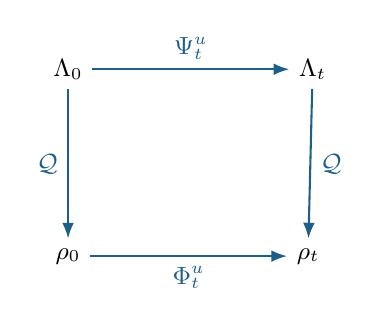
\begin{tikzpicture}[
node distance=19mm and 25mm,
every node/.style={font=\small},
arr/.style={-{Latex[length=2mm]},line width=0.75pt,color=vdblue}
]
\node (l0) {$\Lambda_0$};
\node[right=of l0] (lt) {$\Lambda_t$};
\node[below=of l0] (r0) {$\rho_0$};
\node[right=of r0] (rt) {$\rho_t$};
\draw[arr] (l0) -- node[above] {$\Psi_t^u$} (lt);
\draw[arr] (l0) -- node[left] {$\cQ$} (r0);
\draw[arr] (lt) -- node[right] {$\cQ$} (rt);
\draw[arr] (r0) -- node[below] {$\Phi_t^u$} (rt);
\end{tikzpicture}
\end{center}

\subsection{What failure would and would not mean}

Court 5 attacks \emph{predictive completeness}, not every possible modification of the accepted dynamics:
\begin{description}
\item[Representational completeness:] is \(\cQ\) one-to-one?
\item[Predictive completeness:] if \(\cQ\) is many-to-one, is every matched fibre operationally gauge for every bounded allowed protocol?
\item[Dynamical correctness:] even if \(\rho\) is sufficient, does Nature obey the accepted quantum law for \(\rho\)?
\end{description}
A global Court-5 no-go would remove the claim that \(\rho\) discards observable deeper information. It would not rule out a modified law
\[
\dot\rho=\mathcal L_{\rm QM}(\rho)
+\varepsilon\mathcal F(\rho,C)
\]
with a one-to-one deeper representation. Nor would a null in weak Markovian circuit QED prove global factorization under strong memory, measurement reversal, rapid reference modulation, temporally ordered probes, or composition.

Three evidentiary levels must not be conflated:
\begin{description}
\item[\(\cE_{\mathrm{sys}}>0\):] the reduced Markov qubit state is insufficient.
\item[Bounded process-model excess:] a preregistered completely positive multi-time comb/process tensor with frozen dimension and memory capacity fails on held-out loops \citep{ChiribellaCombs2008,Pollock2018PRA,Pollock2018PRL,Taranto2019,White2022}. Initial correlations and reduced-dynamics domain assumptions remain relevant \citep{Pechukas1994}.
\item[Beyond-quantum claim:] all physically admissible quantum enlargements, including reference and environment memory, are excluded. Finite laboratory characterization cannot literally enumerate an unbounded environment; such a claim requires bounded-resource assumptions or device-independent inequalities.
\end{description}
This hierarchy prevents a memory effect from being mislabeled as a failure of quantum mechanics.

\subsection{Outcome ladder and search order}

\begin{table}[H]
\centering
\small
\begin{tabularx}{\linewidth}{@{}p{0.10\linewidth}p{0.31\linewidth}X@{}}
\toprule
Level & Mathematical result & Scientific status\\
\midrule
A & Derive \(\rho=\cQ(\xi,R,E)\) and recover quantum predictions. & Explanatory reconstruction.\\
B & Prove \(\cQ\) is many-to-one. & Representational redundancy; not new physics.\\
C & Establish matched, protocol-bounded \(V^\star>0\). & The declared reduced quantum state/process model is predictively incomplete.\\
D & If C fails, establish \(P_{\rm alt}(O\mid\rho,a)\neq P_{\rm accepted}(O\mid\rho,a)\). & State sufficient; a modified-dynamics candidate is required and must be tested separately.\\
E & Both C and D fail over the tested domain. & The declared quantum models remain adequate there; Voss Dynamics is explanatory/methodological.\\
\bottomrule
\end{tabularx}
\end{table}

The search order is
\[
\text{single system}
\longrightarrow
\text{temporal process}
\longrightarrow
\text{system+reference}
\longrightarrow
\text{composites}
\longrightarrow
\text{Bell/network scenarios}.
\]
Single-system factorization does not imply composite factorization. A shared reference may support a relational variable
\(C(\Lambda_A,\Lambda_B,R)\)
that is absent from the product of local reduced states. Conversely, any composite proposal must satisfy the no-signalling and Bell constraints already stated. Only a no-go theorem across the declared hierarchy closes the strong predictive-incompleteness branch.

\section{Court 6: freeze, measure, and score}

\subsection{Minimal apparatus}

The target needs one high-coherence qubit, phase-coherent control capable of a closed ray loop, and a nominally \(Z\)-QND readout. A superconducting transmon is natural because dispersive readout, quadrature backaction, trajectory validation, and non-Markovian characterization are mature \citep{Gambetta2008,Hatridge2013,Murch2013,White2022}; it is difficult because strong dispersive readout also causes state mixing and level-dependent effects \citep{Boissonneault2009}. The experiment has five temporal blocks:
\begin{enumerate}
\item prepare the same equatorial state \(\rho_0\);
\item randomly assign \(C_+\), \(C_-\), or a sham loop;
\item close the ray loop and verify final-state equality on a tomography subset;
\item actively reset or characterize the cavity/reference state;
\item acquire a short nominally \(Z\)-QND record with no Rabi drive.
\end{enumerate}

\subsection{Draft calibration and synthetic target}

Independently calibrate \(a\), \(z_0\), readout noise, loop solid angle, the reference offset \(\Gamma_{{\rm rel},0}\), dynamical phase cancellation, leakage, cavity ringdown, and control transfer functions. The illustrative software test fixes \(\Gamma_{{\rm rel},0}=0\). Use only a designated calibration set of solid angles \(\{\Omega_j^{\rm cal}\}\) to estimate \(\varepsilon\):
\begin{equation}
  \widehat\varepsilon
  =
  \arg\min_\varepsilon
  \sum_{j\in\mathrm{cal}}
  \frac{
  [\widehat\Delta_j+2a\varepsilon(1-z_0^2)\sin(\Omega_j/2)]^2
  }{\sigma_j^2}.
  \label{eq:epsilon-fit}
\end{equation}
Then freeze
\begin{equation}
  \Delta_j^{\rm frozen}
  =
  -2a\widehat\varepsilon(1-z_0^2)\sin(\Omega_j^{\rm hold}/2)
  \label{eq:frozen}
\end{equation}
before revealing any held-out record. The repository contains a machine-readable \emph{synthetic} freeze specification and a reproducibility manifest. Regenerating that manifest is not an external timestamped commitment; a physical study requires an independent registry or cryptographic timestamp before acquisition.

\subsection{Likelihood and baselines}

The intended primary score is held-out path likelihood with no refitting. The current code implements only a cell-level integrated-current Gaussian summary score with propagated calibration covariance; it is a software smoke test, not the final path analysis. A confirmatory implementation must compare:
\begin{enumerate}[label=(M\arabic*)]
\item \textbf{Memoryless reduced-qubit null:} \(\varepsilon=0\).
\item \textbf{Bounded calibrated quantum process tensor:} completely positive multi-time model with frozen time grid, intervention basis, memory length/bond dimension, regularization, and confidence set.
\item \textbf{VD-Hopf-1:} the one-parameter frozen sine law.
\item \textbf{Artifact baselines:} pulse energy, duration, signed amplitude leakage, cavity residue, IQ imbalance, thermal drift, and flexible low-rank history models.
\end{enumerate}
Model selection reports predictive log likelihood and complexity separately. Minimum description length is a model-selection rule, not a collapse mechanism. The capacity of every flexible history model must be bounded before target reveal; an unrestricted history model can reproduce the sine law exactly.

\subsection{Power}

In the short-probe approximation, a single rate estimate \(Y_T/T\) has variance \(1/T\). With \(N\) records per orientation,
\[
\operatorname{SE}(\widehat\Delta)=\sqrt{\frac{2}{NT}}.
\]
For one-sided threshold \(z_\alpha\) and power \(1-\beta\),
\begin{equation}
  N
  \ge
  \frac{2(z_\alpha+z_{1-\beta})^2}
  {4a^2\varepsilon^2(1-z_0^2)^2T
  \cos^2\Gamma_{{\rm rel},0}\sin^2(\Omega/2)}.
  \label{eq:power}
\end{equation}
At \(5\sigma\), 90\% oracle power, \(a=1\), \(z_0=0\), \(\Gamma_{{\rm rel},0}=0\), \(T=0.05\), \(\Omega=\pi\), and \(|\varepsilon|=0.02\), the independent-white-noise approximation requires roughly \(9.86\times10^5\) records per orientation. This excludes calibration uncertainty, nuisance estimation, autocorrelation, drift blocks, multiplicity, exclusions, tomography, and process-model comparison; full simulation-based power will be larger.

\begin{figure}[H]
\centering
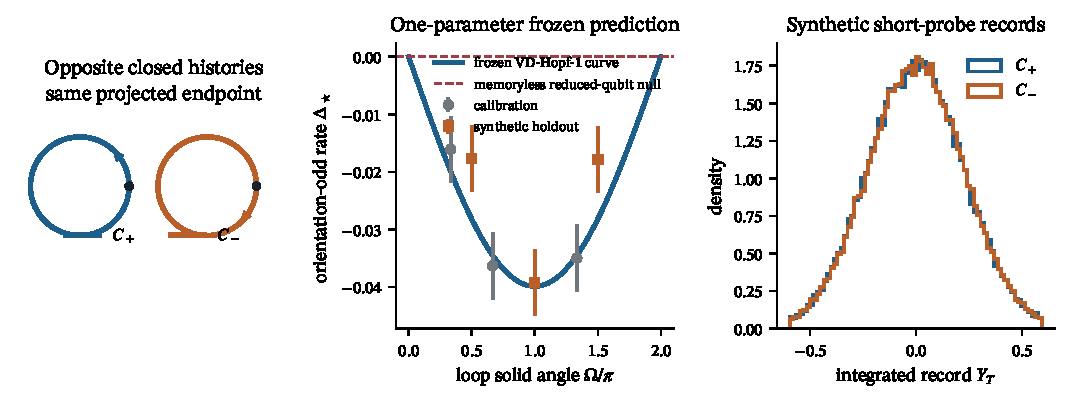
\includegraphics[width=\linewidth]{tiny_target.pdf}
\caption{The tiny target. Closed histories have the same projected endpoint by construction, the one-parameter ansatz freezes a solid-angle sine curve, and synthetic summaries exercise the regression code. The points are synthetic and do not validate a physical memory carrier, complete instrument, or process-tensor comparison.}
\label{fig:tiny-target}
\end{figure}

\begin{figure}[H]
\centering
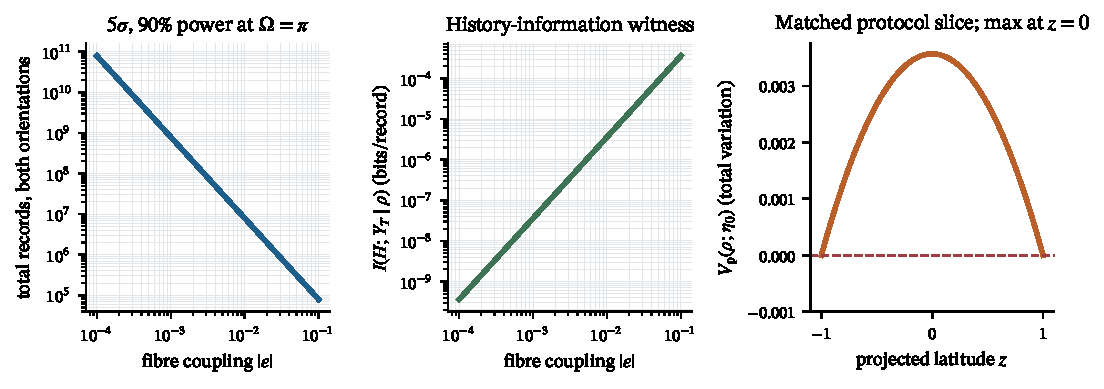
\includegraphics[width=0.9\linewidth]{power_and_information.pdf}
\caption{Left: oracle record cost for \(5\sigma\) and 90\% power. Center: binary-history mutual information per record. Right: the matched protocol-level variation \(V_{\mathsf p}(\rho;\eta_0)\), maximized at the equator. All panels are calculations inside the short Gaussian ansatz.}
\label{fig:power}
\end{figure}

\subsection{Controls}

The following controls are mandatory:
\begin{itemize}
\item \textbf{Final-state equivalence:} a one-sided equivalence test using SPAM-robust tomography or gate-set tomography bounds the trace distance tightly enough that the largest permitted \(z_+-z_-\) cannot explain the target. At the illustrative \(a=1,\varepsilon=0.02,\Omega=\pi\) point, a \(0.04\) population mismatch reproduces the entire leading rate difference. Randomized benchmarking is auxiliary and cannot establish state equality.
\item \textbf{Leakage:} characterize at least the qutrit populations and level-dependent IQ response; equality of normalized \(2\times2\) blocks is insufficient.
\item \textbf{Dynamical phase:} freeze explicit \(H_\pm(t)\), calculate the dynamical phase, reconstruct the realized state path, and set a numerical residual-phase margin. ``Use echo'' is not a complete protocol.
\item \textbf{Ringdown:} measure complex cavity amplitude and covariance, not photon number alone; vary delay and fit a frozen multi-mode ringdown model.
\item \textbf{Sham and zero-area loops:} equal pulse count, energy, and duration with \(\Omega=0\) must be null.
\item \textbf{Orientation swaps:} cable/IQ labels, pulse compilation, and readout sign are independently reversed.
\item \textbf{Loop families:} geometrically distinct paths with the same \(\Omega\) must agree; equal-duration paths with different \(\Omega\) must follow the sine law.
\item \textbf{Process tensor:} freeze time grid, intervention basis, leakage dimension, memory length/bond dimension, regularization, stationarity assumptions, confidence set, and out-of-distribution rule.
\item \textbf{Replication:} repeat with a second control implementation and independent analysis team.
\end{itemize}

\subsection{Hard pass/fail rule}

The draft is not executable until it has: a mixed-state or bias-qualified pure-state extension; a minimum composable instrument-consistency result; explicit control Hamiltonians and reset law; implemented path score; validated bounded qutrit--cavity and process-tensor nulls; numeric thresholds, sample count, autocorrelation correction, missing-data rules, and equivalence margins; frozen model capacities; and an external commitment. Only after those blockers are closed can VD-Hopf-1 enter a bounded-model laboratory stage, where:
\begin{enumerate}
\item the frozen held-out likelihood exceeds the memoryless reduced-qubit, qutrit--cavity, and declared finite-memory models by the preregistered threshold;
\item the full solid-angle, orientation, \(z_0\), delay, and reference-phase dependence is jointly correct;
\item no post-unsealing parameter change is made;
\item every equivalence and negative-control margin holds; and
\item the bounded calibrated process-tensor prediction fails outside its frozen confidence set.
\end{enumerate}
Independent replication is a separate confirmation stage. Even a single-stage pass establishes unexplained history dependence relative to the listed bounded models, not exclusion of all enlarged quantum models. If \(\widehat\varepsilon\) is consistent with zero, VD-Hopf-1 is bounded or rejected at the achieved scale; the conditional scalar characterization and QND coordinate method may remain.

\section{Computational evidence}

\subsection{Reproducible suite}

The evidence package performs:
\begin{enumerate}
\item symbolic verification of both It\^o residuals for the QND invariant and quotient;
\item the integer scalar-selection calculation \(2=1+d(d-1)/2\);
\item positivity, trace, and global-phase invariance tests for \(\cQ\);
\item Born trace identities on random Bloch states;
\item unitary invariants, dephasing, Rabi, and Zeno calculations;
\item singlet correlations, \(2\sqrt2\) CHSH, and no-signalling marginals;
\item deformation symmetry tests;
\item algebraic invariance of \(\psi\psi^\dagger\) under inserted opposite phases (not a loop/control simulation);
\item an ordinary-quantum coherent-memory countermodel with equal photon number and nonzero homodyne distinguishability;
\item direct evaluation of \(V_{\mathsf p}(\rho;\eta_0)\) and \(V^\star_{\mathsf p,\eta_0}\) in the short-probe candidate;
\item frozen synthetic calibration/holdout scoring, power, and mutual information.
\end{enumerate}

The automated test suite passes all unit tests. Representative maximum errors are \(2.3\times10^{-16}\) for Born probabilities, \(7.8\times10^{-16}\) for Rabi evolution, \(1.2\times10^{-16}\) for no-signalling marginals, and below \(5\times10^{-16}\) for global-phase projection. These are floating-point checks of exact identities.

\subsection{What the synthetic freeze proves}

Synthetic Gaussian summaries generated from VD-Hopf-1 show that the calibration--freeze--reveal regression can recover a small coupling and predict held-out angle cells without refitting. They do not validate path likelihood, a complete instrument, or process-tensor discrimination. Because the simulator contains the fitted functional family, this is a software/protocol smoke test only.

\section{Impact if the program succeeds}

\subsection{A physical origin for complex structure}

\Cref{thm:complex-scalar} offers a conditional dimension criterion for a familiar mathematical fact. A real stationary reference produces a quarter-turn operator \(J_R^2=-I\); its two-dimensional span matches the complete unnormalized binary QND-filter algebra only at Peirce degree two. If the accessibility and response-completeness premises can be derived from weaker coupling principles, the criterion could contribute to explaining why complex amplitudes are selected.

\subsection{A sharper meaning of ``emergent''}

The map \(\cQ\) is not a decoder metaphor. It is an explicit quotient:
\[
\text{real normalized spinor and reference}
\longrightarrow
\text{complex ray/density matrix}
\longrightarrow
\text{operational predictions}.
\]
The fibre distinction identifies what the redundant pure-spinor lift retains and what \(\rho\) identifies. Standard quantum mechanics declares the global \(U(1)\) direction gauge. VD-Hopf-1 postulates a distinct closed-history carrier and asks whether a residual relation predicts a later record after a bounded matched reset. A positive result would first establish insufficiency of the declared reduced-state/process model, not immediate failure of all quantum theory.

\subsection{Measurement and randomness}

The QND chart shows that a real measurement record can drive both information gain and phase backaction along one trajectory while leaving a transverse state label conserved. This is standard quantum filtering, but the chart makes the quotient geometry constructive. If a fibre coupling existed, some apparent measurement randomness would become conditionally structured by \(\Gamma_{\rm rel}\). That would not make outcomes globally deterministic without a complete environment law; it would show only that \(\rho\) omitted predictive information.

\subsection{Quantum engineering}

Even a null result can be useful. The protocol measures how well a reduced qubit state or calibrated process tensor predicts records after closed loops. It therefore probes coherent pulse memory, cavity reset, geometric control, and low-rank non-Markovian structure. The supplied observability search also yields a principled single-meter control design, though continuous one-axis tomography with Rabi control is established \citep{Chantasri2019}. The engineering contribution is disciplined model discrimination, not a new detector.

\subsection{Scientific method}

The most transferable contribution is the chain
\[
\boxed{
\text{derive}\ \longrightarrow\
\text{commit}\ \longrightarrow\
\text{measure}\ \longrightarrow\
\text{score}\ \longrightarrow\
\text{replicate}.
}
\]
Foundational claims are unusually vulnerable to flexible reinterpretation. A symmetry-truncated deformation, externally committed target, bounded adversarial quantum-memory null, machine-readable constants, and hard loss condition can convert an interpretive proposal into an experiment that can say ``no.'' The present repository prepares that workflow but is not itself an externally registered physical study.

\section{Limitations and open theorems}

\begin{enumerate}
\item \textbf{The EJA premise is not derived.} Homogeneity, self-duality, finite dimensionality, and irreducibility delimit the theorem.
\item \textbf{Generator completeness is an axiom.} It may be physically motivated, but it currently performs the decisive scalar selection.
\item \textbf{The reference-to-state relation is not unique.} \(J_R^2=-I\) gives a complex structure; identifying the same reference with every system phase requires a coupling law.
\item \textbf{The holonomy carrier is postulated.} A path functional is not automatically an endpoint state coordinate; retaining it while matching the full standard quantum process state is the decisive conjecture.
\item \textbf{The Hopf coupling is conjectural.} The sine term is one selected finite-basis element, not a symmetry-unique law.
\item \textbf{Global phase is ordinarily gauge.} A physical reference enlarges the quantum system and can turn apparent global phase into standard relative phase. The experiment must beat the declared bounded enlarged-quantum null.
\item \textbf{The ansatz is pure-state and noncomposable.} No canonical mixed-state holonomy, completely positive instrument, qutrit extension, or adaptive multipartite law is derived.
\item \textbf{A local model is not a composite theory.} No-signalling, Bell correlations, and preparation contextuality must coexist in a complete multipartite extension.
\item \textbf{Finite process tomography is bounded.} Failure of a chosen process-tensor model is not logical exclusion of every quantum environment.
\item \textbf{The protocol is not yet executable.} Numeric decision thresholds, capacity bounds, path likelihood, qutrit--cavity simulations, equivalence margins, and an external commitment remain.
\item \textbf{No laboratory result is included.} The thesis reaches a conditional-theorem and candidate-protocol milestone, not physical confirmation.
\end{enumerate}

\section{Conclusion}

The six courts force the broad idea of Emergent Predictive Representation into a small and auditable statement.

The conditional reconstruction begins with operational convexity, a Jordan-domain assumption, strengthened measure-preserving or Hamiltonian dynamics, and a stationary real detector reference. The reference span has two real directions. A binary Jordan face has \(1+d(d-1)/2\) unnormalized QND filter directions. The dimension-forcing response axiom selects \(d=2\), conditionally recovering complex quantum scalars.

The effective pure-qubit map can be represented by the redundant Hopf lift \(\psi\mapsto\psi\psi^\dagger\). The ideal QND equations become a straight translation in \((s,\vartheta)\), but their conserved transverse coordinate remains encoded in \(\rho\). The chosen normalized-spinor lift has a \(U(1)\) fibre; promoting a closed-history relation on that fibre to physical memory is an explicit candidate postulate, not a consequence of quantum-state geometry.

The leading orientation-odd candidate readout correction is
\[
\dd Y_t
=a[z_t+\varepsilon(1-z_t^2)\sin\Gamma_{{\rm rel},t}]\dd t+\dd W_t,
\]
and its frozen small-target signature is
\[
\Delta_\star(\Omega)
\simeq-2a\varepsilon(1-z_0^2)
\cos\Gamma_{{\rm rel},0}\sin(\Omega/2)
\]
Equivalently, the direct candidate optimization gives
\[
V^\star_{\mathsf p,\eta_0}
\simeq2\Phi(a|\varepsilon|\sqrt T)-1.
\]
The repository specifies a draft calibration, holdout, Gaussian summary score, power calculation, controls, hashes, and qualitative failure rules. It does not yet implement the bounded process-tensor and qutrit--cavity nulls needed before a confirmatory run. If a genuine adaptive factorization theorem instead forces all matched protocol variations to zero, the claim that \(\rho\) discards observable deeper information is closed cleanly; the conditional complex-scalar characterization survives, and a logically separate modified-\(\rho\) dynamics branch remains available. The scientifically credible conclusion today is that a one-parameter phenomenological target and explicit theory/protocol closure conditions have been isolated for further work.

\appendix

\section{Full matrix proof of the unnormalized QND-filter stabilizer}
\label{app:stabilizer}

Use coordinates \(v=(t,z,\bm c)\) and Lorentz metric
\(\eta=\operatorname{diag}(1,-1,-I_d)\).
Modulo a scalar dilation, an infinitesimal cone automorphism \(X\) obeys
\[
X^\mathsf T\eta+\eta X=0.
\]
Write
\[
X=
\begin{pmatrix}
a & b & \bm u^\mathsf T\\
c & d & \bm v^\mathsf T\\
\bm p & \bm q & M
\end{pmatrix}.
\]
The Lorentz condition gives \(a=d=0\), \(b=c\), \(\bm p=\bm u\), \(\bm q=-\bm v\), and \(M^\mathsf T=-M\). Preserving each ray generated by \(n_\pm=(1,\pm1,\bm0)\) requires
\[
Xn_\pm\in\operatorname{span}(n_\pm).
\]
The transverse components are \(\bm p\pm\bm q\), so both vanish and hence \(\bm p=\bm q=\bm u=\bm v=\bm0\). The remaining matrix is
\[
X=
b
\begin{pmatrix}
0&1&0\\
1&0&0\\
0&0&0
\end{pmatrix}
+
\begin{pmatrix}
0&0&0\\
0&0&0\\
0&0&M
\end{pmatrix},
\qquad M\in\mathfrak{so}(d),
\]
which proves \cref{eq:qnd-algebra}. Stabilizing only one null ray would leave null rotations; stabilizing both is essential.

\section{It\^o derivation of the relational QND chart}
\label{app:ito}

For \(s(z)=\artanh z\),
\[
s'(z)=\frac{1}{1-z^2},
\qquad
\frac12s''(z)=\frac{z}{(1-z^2)^2}.
\]
Using \cref{eq:qnd-z},
\[
(\dd z)^2=a^2\cos^2\varphi(1-z^2)^2\dd t.
\]
Therefore
\begin{align*}
\dd s
&=s'(z)\dd z+\frac12s''(z)(\dd z)^2\\
&=a\cos\varphi\,\dd W
+a^2\cos^2\varphi\,z\,\dd t\\
&=a\cos\varphi\,\dd Y.
\end{align*}
Substitution of \cref{eq:qnd-record} into \cref{eq:qnd-theta} likewise gives
\(\dd\vartheta=a\sin\varphi\,\dd Y\). The orthogonal rotation to \((x_\varphi,c_\varphi)\) then yields \cref{eq:qnd-translation}. The symbolic evidence suite differentiates the candidate first integral directly and verifies both its diffusion and drift residuals are identically zero.

\section{Why exact QND apparatus readout is phase blind}
\label{app:phase-blind}

An exact \(Z\)-QND system--environment unitary has controlled form
\[
U
=\proj{0}\otimes U_0+\proj{1}\otimes U_1.
\]
For
\(\ket{\psi}=\alpha\ket0+\beta\ket1\)
and an initially uncorrelated, preparation-phase-independent environment state
\(\proj{\psi}\otimes\rho_E\), tracing out the qubit after interaction gives
\[
\rho_E'
=|\alpha|^2U_0\rho_EU_0^\dagger
+|\beta|^2U_1\rho_EU_1^\dagger.
\]
The cross terms vanish because
\(\Tr_S(\ket0\!\bra1)=0\).
Hence every environment-only POVM has probabilities independent of
\(\arg(\alpha^\ast\beta)\). No nonlinear statistic of that exact apparatus-only record can recover the initial relative phase. A drive, non-QND term, unrecovered cavity mode, or joint system--environment recombination can reveal phase within standard quantum mechanics; those are different experiments.

\section{Deformation expansion beyond leading order}
\label{app:deformation}

The general smooth reference-covariant, mirror-odd correction is
\[
g(z,\Gamma_{\rm rel},\mathsf h)
=
\sum_{n\ge1}f_n(z,\mathsf h)\sin(n\Gamma_{\rm rel}),
\]
where \(\mathsf h\) denotes causal history features. Sharp eigenstate calibration imposes \(f_n(\pm1,\mathsf h)=0\). For an analytic static model,
\[
f_n(z)
=(1-z^2)
\sum_{k\ge0}
\left(a_{nk}z^{2k}+b_{nk}z^{2k+1}\right).
\]
Additional branch-relabel and time-reversal conventions determine whether the \(a\)- or \(b\)-sector survives. VD-Hopf-1 keeps \(a_{10}=\varepsilon\) and sets all other coefficients to zero before target data. An experimental rejection can therefore mean either \(\varepsilon=0\) or that this truncation is wrong; it does not reject every conceivable history-dependent model.

\section{Likelihood, information, and power}
\label{app:statistics}

For equal priors and the short Gaussian pair
\[
Y\mid H=\pm\sim\mathcal N(\pm m,T),
\]
the log likelihood ratio is \(2mY/T\). The mutual information in bits is
\[
I(H;Y)
=1-\E_{Z\sim\mathcal N(0,1)}
\log_2\!\left[
1+\exp\!\left(
-\frac{2m(m+\sqrt T Z)}{T}
\right)
\right].
\]
The evidence code evaluates this integral by Gauss--Hermite quadrature. At small \(m^2/T\), information is quadratic in \(\varepsilon\), matching the inverse-square sample cost in \cref{eq:power}.

For held-out integrated records \(y_i\) with known variances \(T_i\), the primary Gaussian score is
\[
\ell(M)
=-\frac12\sum_i
\left[
\frac{(y_i-\mu_i^{M})^2}{T_i}
+\log(2\pi T_i)
\right].
\]
All preprocessing, exclusions, covariance corrections, and stopping rules must be frozen with the model.

\section{Reproducibility map}
\label{app:reproducibility}

\begin{table}[H]
\centering
\small
\begin{tabularx}{\linewidth}{@{}p{0.31\linewidth}X@{}}
\toprule
Artifact & Purpose\\
\midrule
\path{evidence/epr_core.py} & Relational map, Hopf projection, Jordan dimension, quantum limits, target law, power, and simulation.\\
\path{evidence/run_all.py} & Deterministic end-to-end evidence generation and all thesis figures.\\
\path{evidence/tests/test_epr_core.py} & Unit tests for positivity, fibre invariance, QND chart, Born/CHSH/no-signalling, deformation symmetries, and shot scaling.\\
\path{evidence/outputs/metrics.json} & Machine-readable numerical results and evidence status.\\
\path{evidence/outputs/frozen_prediction.json} & Candidate version, formula, calibration constants, held-out angles, and primary score.\\
\path{evidence/outputs/manifest.sha256} & Hashes of code and generated evidence artifacts.\\
\path{blind_qnd_research.py} & Supplied independent symbolic and observability-discovery seed calculation.\\
\bottomrule
\end{tabularx}
\end{table}

From the repository root:
\begin{verbatim}
uv sync --all-groups
uv run pytest
uv run python -m evidence.run_all
tectonic -X compile thesis/main.tex --outdir thesis/build
\end{verbatim}
The random seed is fixed at \(20260821\). Generated target records are explicitly marked synthetic in every machine-readable output.

\section{Court-by-court falsification matrix}

\begin{table}[H]
\centering
\small
\begin{tabularx}{\linewidth}{@{}p{0.08\linewidth}p{0.31\linewidth}X@{}}
\toprule
Court & Pass object & Failure condition\\
\midrule
1 & Correct conditional classification with explicit axioms. & Counterexample to the reference theorem, stabilizer lemma, or EJA classification step; hidden dimensional assumption.\\
2 & Positive normalized \(\cQ\), exact chart, correct fibres. & A claimed lost variable is reconstructible from \(\rho\), or reference structure is merely renamed complex notation.\\
3 & Exact \(\varepsilon=0\) quantum laws and composites. & Failure of positivity, Born calibration, CP baseline, CHSH, or no-signalling.\\
4 & Frozen symmetry basis and remainder class. & A lower-order allowed term was omitted, or target term violates a declared symmetry.\\
5 & Same \(\rho\), different \(\Lambda\), nonzero candidate separation. & Preparation arms end in distinguishable \(\rho\), or predicted difference vanishes identically.\\
6 & Sealed held-out likelihood and independent replication. & Post-hoc fitting, process-memory explanation, control failure, null result, or non-replication.\\
\bottomrule
\end{tabularx}
\end{table}

\bibliographystyle{unsrtnat}
\bibliography{references}

\end{document}
